\chapter{Cómputo bayesiano}

De acuerdo con \textcite{Ross10}, los resultados más importantes y más conocidos de la teoría de probabilidad son los llamados teoremas límite, en particular aquellos conocidos como \textit{leyes de los grandes números}. La idea general podemos tomarla de Jakob Bernoulli, el primero en presentar un teorema de este tipo, y estriba en que todos los hombres saben ``por algún instinto de la naturaleza \textit{per se} y sin ninguna instrucción previa, que entre más observaciones hay, menor es el peligro de alejarse del blanco" \parencite{Pulskamp09}. Es decir, si tenemos suficientes realizaciones de un experimento, podemos estimar con mucha precisión aquello que buscamos. Así, después de varios avances históricos que pueden consultarse en \textcite{Seneta13}, hoy tenemos las siguientes dos leyes generales de los grandes números, cuyas pruebas bajo algunos supuestos adicionales pueden consultarse en \textcite{Ross10}:

\begin{teo} \label{teo:LGN}
\textbf{Leyes de los grandes números.}
Sean $X_1,\,X_2,\dots$ una secuencia de variables aleatorias independientes e idénticamente distribuidas, cada una con media finita $E[X_i]=\mu$, y $\bar{X}_N=\sum\limits_{i=1}^N\dfrac{X_i}{N}$, las respectivas medias empíricas. Entonces se cumplen las siguientes dos leyes.\\ 
\begin{itemize}
\item \textbf{Ley débil}
\begin{equation*}
\lim_{N \to \infty} P\left( |\bar{X}_N-\mu| \geq \epsilon \right)  = 0 \qquad \forall \, \epsilon > 0
\end{equation*}
\item \textbf{Ley fuerte}
\begin{equation*}
P\left(\lim_{N \to \infty} \bar{X}_M = \mu \right)  = 1 
\end{equation*}
\end{itemize}
\end{teo}

Ambas leyes nos dicen que, conforme el tamaño de una muestra aleatoria aumenta, los promedios empíricos convergen a los promedios teóricos. Una manera común de ejemplificar este fenómeno es mediante el lanzamiento sucesivo de monedas. En este caso los volados \textit{simulan} observaciones de una variable aleatoria de ensayos Bernoulli y, al tener una muestra suficientemente grande, se comienza a apreciar la convergencia hacia la probabilidad de éxito. Gracias al avance tecnológico, hoy ya no tenemos necesariamente que lanzar volados físicamente sino que los simulamos desde una computadora, a partir de la generación de números pseudoaleatorios, diseñados de manera tal que satisfagan todas las propiedades básicas de números auténticamente aleatorios \parencite{Ross13}. Podemos pedirle a la computadora que simule una gran cantidad de volados y registre la proporción empírica acumulada de los que cayeron águila. Conforme más aumenta el número de volados, más nos acercamos a 0.5, la proporción teórica. Esto se puede repetir para otras series de volados y el comportamiento es el mismo, como puede apreciarse en la \ref{fig:LGN}. \\

\begin{figure}[h]
	\centering
	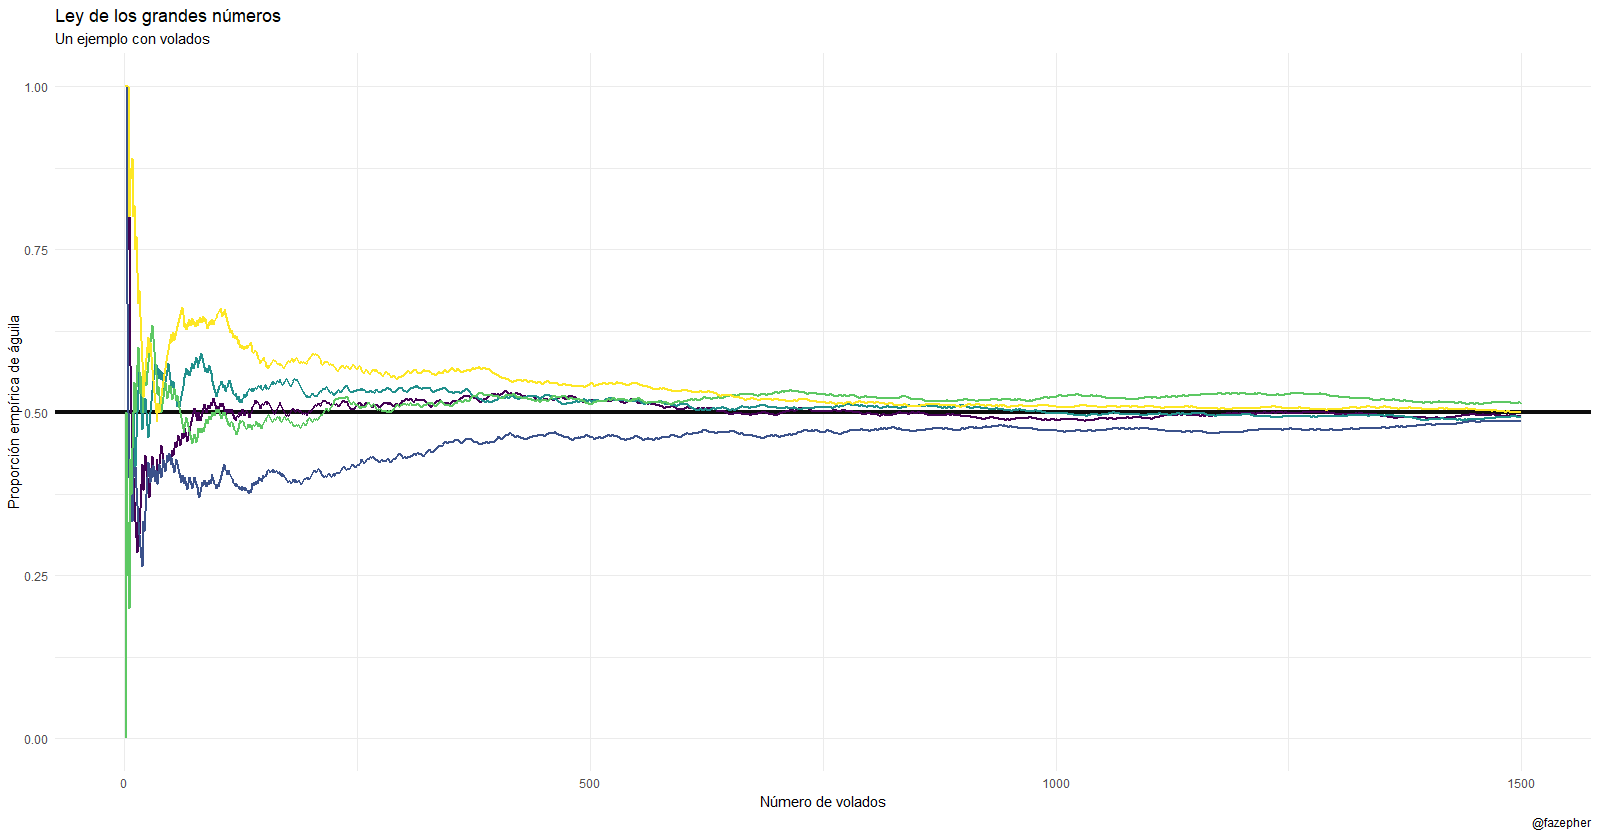
\includegraphics[scale=0.25]{Figs/LGN}
	\caption{Ilustración de las leyes de los grandes números mediante volados simulados por computadora. Conforme el número de volados aumenta, la proporción empírica converge a la proporción teórica. Esto pasa para cada serie de volados. Fuente: elaboración propia.}
	\label{fig:Regimen_Semipresidencial_VRepFr}	
\end{figure}

Es cierto que esta práctica de aprender de un sistema, simulando con muestreo aleatorio no surge con las computadoras \parencite{Owen13}. Ya desde 1812 Laplace había sugerido la posibilidad de estimar empíricamente el valor de $\pi$ mediante el llamado problema de la aguja de Buffon \parencite{Ragheb13}. Sin embargo, como el ejemplo de los volados muestra, sí han sido las computadoras las que han potenciado la utilidad de los métodos de simulación. ¿Cuánto hubiéramos tardado en lanzar los 7,500 volados que la computadora simuló al instante? Más aún, esta capacidad computacional consolidó la utilidad de la estadística bayesiana. ¡Y pensar que todo empezó con una guerra y un juego de solitario!, como explico a continuación.

\section{Monte Carlo} 

La simulación por computadora ha permitido el desarrollo de la estadística bayesiana, particularmente desde la década de los 90 del siglo pasado \parencite{RobertCasella11}. Sin embargo, la semilla de este desarrollo ya había sido plantada medio siglo antes desde el terreno de la física, desafortunadamente a causa de la Segunda Guerra Mundial, por los científicos del laboratorio de Los Alamos, encargados del proyecto Manhattan y el desarrollo de más armas de fisión nuclear.\\

Uno de esos científicos fue un matemático polaco-estadounidense llamado Stanislaw Ulam. En 1946, aburrido convaleciendo por una enfermedad, comenzó a preguntarse sobre la probabilidad de ganar en un juego de solitario. Después de mucho batallar con los cálculos de combinatoria se planteó si no sería más práctico estimarla simulando muchas partidas en una de las primeras computadoras electrónicas. Y ahí surgió el eureka: ¿por qué no hacer lo mismo para los problemas de física nuclear en los que estaban trabajando en Los Alamos? \parencite{Eckhardt87}. Al igual que las partidas de solitario, podrían simular muchas realizaciones de los procesos físicos bajo estudio y estimar los resultados más probables.\\ 

Stan compartió su idea con John von Neumann quien, sorprendido y emocionado con la idea, le envió una carta a Richard Richtmayer--- el líder del equipo en Los Alamos--- con todos los cálculos necesarios para llevar a cabo el proyecto \parencite{vonNeumann47}. El método fue rápidamente adoptado por todos en Los Alamos, tanto que otro físico, Nicholas Metropolis, sugirió llamarlo \textit{Monte Carlo}, bromeando sobre un tío apostador de Stan, que vivía pidiendo prestado dinero porque ``simplemente tenía que ir a Monte Carlo" \parencite{Metropolis87}. Después de un arduo trabajo, el método pareció funcionar--- gracias en buena medida al trabajo de programación de Klara von Neumann \parencite{Haigh14}--- y el propio Metropolis publicó, junto con Stan, un primer paper presentándolo a grandes rasgos \parencite{MetropolisUlam49}.\\

De manera concreta, el método es la conjunción de la simulación con la ley de los grandes números. Al fin y al cabo, las cantidades que requerían calcular eran valores esperados de la siguiente forma: 
\begin{equation*}
\bar{h} = \mathbb{E}[h(q)]=\int\limits_\mathcal{Q} h(q)f(q)dq ,
\end{equation*} 
donde $h$ es una función de interés y $f(q)$ es la distribución de probabilidad sobre las \textit{configuraciones} en las que podía encontrarse el sistema físico. Estas integrales típicamente no pueden calcularse ni analíticamente ni por métodos numéricos tradicionales. Sin embargo, si se tiene una muestra aleatoria de valores de $q$ provenientes de su distribución $f$, se podría aproximar $\bar{h}$ con el promedio empírico: 
\begin{equation*}
\bar{h} \approx \sum\limits_{i=1}^N \dfrac{h(q_i)}{N}
\end{equation*}

Esta forma aparentemente sencilla conlleva una gran flexibilidad de \textit{resúmenes inferenciales} que se pueden llevar a cabo. Por lo que la posibilidad de realizar la \textit{integración por Monte Carlo}, hace que en la práctica exista una dualidad entre una distribución o densidad y una muestra proveniente de ella \parencite{SmithGelfand92}. El problema para los científicos en Los Alamos se convirtió entonces en encontrar algoritmos eficientes para obtener una muestra aleatoria de variables que seguían diferentes distribuciones $f$.

\section{Metropolis-Hastings}

Aunque se fueron desarrollando métodos de simular de manera independiente variables aleatorias, no todas las distribuciones 

\begin{itemize}
\item Queremos una muestra suficientemente grande de la posterior. Para ello requerimos un método que genere una realización \textit{independiente} de la posterior. 

\item Una distribución límite de una Cadena de Markov es tal que no cambia. Esto quiere decir que si una simulación de una cadena de Markov llega a la distribución límite, cada nueva simulación se genera de manera independiente. 

\item Si no conozco completamente una distribución posterior, ¿existe alguna cadena de Markov cuya distribución límite sea esta distribución posterior? Si existiera entonces podría simular la cadena y, eventualmente, llegar a la distribución límite y, entonces, ya podría simular una muestra aleatoria de mi distribución posterior.

\item Una muestra suficientemente grande de esta distribución posterior satisface la única receta. Los resúmenes de Monte Carlo permiten la inferencia axiomática, por llamarla de una manera.  
\end{itemize}




